\chapter{Literature Review}\label{ch:LitReview}

\section{Context}
In order to understand this thesis, it is import to first understand it's context, in particular why tracking is both critical to the operation of the receiver, as well as why it is so challenging. This chapter aims to provide a broad overview of the relationship between the material covered in this thesis, as well as it's connection to other work covered in the literature. 

\subsection{Challenges}
Using a GPS receiver for \ac{LV} exposes the receiver to some of the most extreme circumstances imaginable. As elicited in table \ref{tab:Requirements}, we can observe that the receiver experiences velocities and accelerations far beyond what would be experienced in terrestrial applications.  The rationale behind these requirements can be found in appendix \ref{ch:FlightDynamics} and \ref{ch:Falcon9}. 
While \ac{GPS} receivers are normally used to provide provide absolute positions, the ability to provide highly accurate velocity data is incredibly valuable for spacecraft guidance. In order to insert a satellite into the proper orbit, the \ac{LV} engine-cutoff must be precisely timed, as orbital height is a function of orbital velocity. Based on analysis carried out in appendix \ref{ch:Falcon9}, we can conclude that the receiver needs to be able to provide velocity solutions which are accurate $\leq 1m/s$, while travelling at 6,000m/s. 

\begin{table}[!htb]
\centering
\begin{tabular}{|l|l|}
\hline
\rowcolor[HTML]{C0C0C0} 
Parameter    & Value                    \\ \hline
Altitude     & 200,000$m$                 \\ \hline
\rowcolor[HTML]{EFEFEF} 
Velocity     & 6,000$m/s$                 \\ \hline
Acceleration & 150$m/s^2$ \\ \hline
\rowcolor[HTML]{EFEFEF} 
Jerk         & 10$m/s^3$  \\ \hline
\end{tabular}
\caption{Receiver operational conditions.}
\label{tab:Requirements}
\end{table}

TALK ABOUT EXPORT CONTROLS
Unfortunately, the requirements of operation exceed the \ac{COCOM} limits, which prevent the export from the USA of GNSS receivers capable of operating:

\begin{itemize}
\item{Above 60,000ft (18,000 m)}
\item{Faster than 1,000 knots (514 m/s) }
\end{itemize}

This helps to explain the motivation to develop a receiver, which is free from \ac{COCOM} requirements.

Due to the relative motion of the satellite and the receiver, the received signal differs from the transmitted carrier frequency of 1575.42 MHz due to the Doppler effect\cite{Tsui}. The frequency offset due to the \ac{LOS} velocity between the receiver and the satellite can be found using \ref{eq:DopplerShift} to be 5.25Hz per m/s. Hence for the velocities experienced by \ac{LV} and \ac{SV}, we can expect Doppler shifts of up to 10's of KHz.

\begin{align}
\Delta f &= f_0\frac{v}{c} \text{ Hz/m/s}
\label{eq:DopplerShift}
\end{align}

Where: 
\begin{align*}
f_0 &= 1575.42 \text{ MHz}\\   
c &= 2.99792458 \times 10^8 \text{ m/s}
\end{align*}


Making reference to table \ref{tab:DopplerDynamics}, we can observe that different orders of motion have differing impacts on the Doppler frequency. In figure \ref{fig:DopplerShift}, we can directly observe the effect of the receiver dynamics on the Doppler shift observed by the receiver.

\begin{figure}[!htb] 
    \centering
    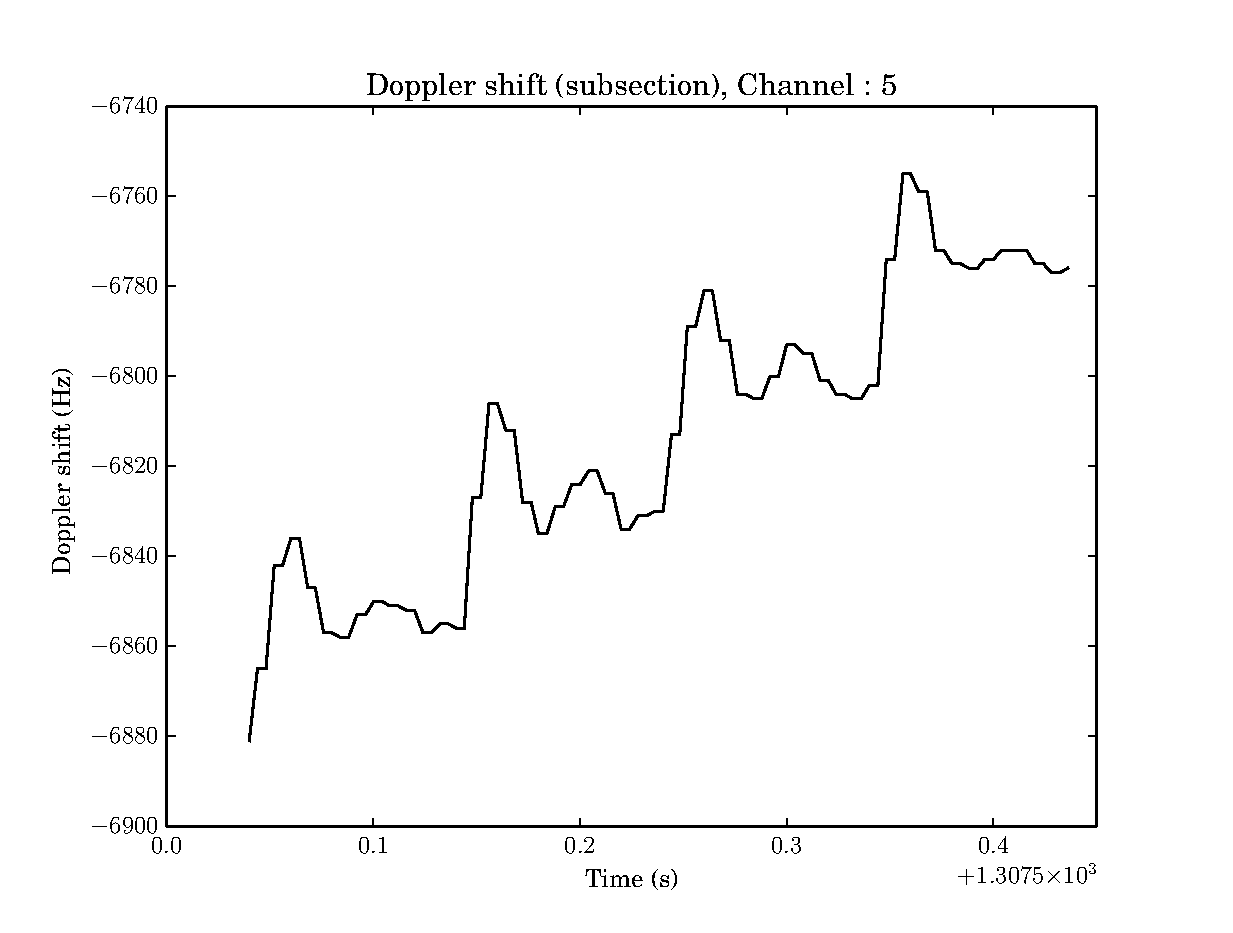
\includegraphics[width=1\textwidth]{LitReview/DopplerShift5.eps} 
    \caption{In this figure, we can observe a ramp in the Doppler frequency of approximately 6,000Hz over 22.5 seconds. From this, we can conclude that the receiver is accelerating at $\approx50 m/s^2$.}
    \label{fig:DopplerShift}
\end{figure}


\begin{table}[!htb]
\centering
\begin{tabular}{|l|l|}
\hline
\rowcolor[HTML]{C0C0C0} 
Change in \ac{LOS} Distance & Doppler frequency \\ \hline
Static                 & 0                 \\ \hline
\rowcolor[HTML]{EFEFEF} 
Velocity               & Constant          \\ \hline
Acceleration           & Ramp              \\ \hline
\rowcolor[HTML]{EFEFEF} 
Jerk                   & Parabolic         \\ \hline
\end{tabular}
\caption{The relationship between \ac{LOS} dynamics and Doppler frequency.}
\label{tab:DopplerDynamics}
\end{table}

Turning our attention to the motion of the GPS satellite, Tsui states that the maximum line of sight velocity for a stationary receiver due to the motion of the satellite is $\approx 929 m/s$, or 4.9KHz. Finally, it is important to note that the maximum \ac{LOS} acceleration due to the motion of the satellite is $\approx 0.188m/s^2$, or 0.936 Hz/s\cite{Tsui}. From this, we can conclude that the \ac{LOS} dynamics are dominated by the motion of the receiver.

\section{Introduction to PLLs}
PLLs are a versatile tool for solving many problems in electrical engineering, hence there is a significant body of literature which relates to the design, implementation and applications of PLLs. 

One of the most beautiful properties of a PLL, is that once it has locked onto an incoming signal, then the average frequency of the local replica is \emph{exactly} equal to the average frequency of the incoming signal. We can understand why this is true, as if the average frequency of the local replica of was different to the average frequency of the incoming signal, than the phase error would increase over time, and eventually the loop would loose lock. This property can be exploited in order to provide an highly accurate estimate of the velocity of the receiver based on the Doppler shift in frequency. As alluded to before, the receiver needs to be able to provide velocity solutions which are accurate to better than 1m/s, or 5.25Hz of Doppler shift. It is important to remember that phase lock does not imply zero phase error, or zero instantaneous velocity error\cite{Gardner}. 

\tikzset{
block/.style = {draw, fill=white, rectangle, minimum height=3em, minimum width=3em},
tmp/.style  = {coordinate}, 
sum/.style= {draw, fill=white, circle, node distance=1cm},
input/.style = {coordinate},
output/.style= {coordinate},
pinstyle/.style = {pin edge={to-,thin,black}
}
}

\begin{figure}[!htb]
\centering
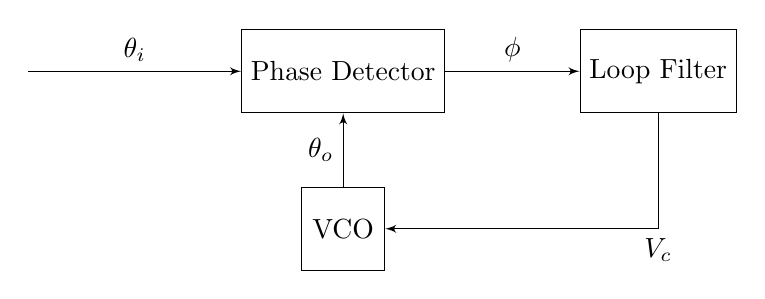
\begin{tikzpicture}[auto, node distance=4cm,>=latex']
    \node [input, name=rinput] (rinput) {};
    
    
    \node [block, right of=rinput](PhaseDetector){Phase Detector};
    
    \node [block, right of=PhaseDetector] (LoopFilter) {Loop Filter};
    
    \node [block, below of = PhaseDetector,node distance = 2
    cm](VCO){VCO};
    
    \draw [->] (rinput) -- node{$\theta_{i}$} (PhaseDetector);
    \draw [->] (PhaseDetector) -- node{$\phi$} (LoopFilter);
    \draw [->] (LoopFilter) |- node{$V_{c}$} (VCO);
    \draw [->] (VCO) -- node{$\theta_{o}$} (PhaseDetector);
    
    \end{tikzpicture}
\caption{An abstracted diagram of a typical PLL.} 
\label{fig:PLLAnalog}
\end{figure}


Every PLL contains 3 key components,

\begin{itemize}
\item{Phase Detector}
\item{Loop Filter}
\item{Oscillator}
\end{itemize}

In figure \ref{fig:PLLAnalog} we can observe relationship between these components. The \emph{Phase Detector} measures the phase between difference an incoming signal $\omega_{input}$ and an internally generated signal $\omega_{local}$, generating the error signal, which is ideally equal to $\theta_i -\theta_o$. This error signal is then filtered by the \emph{Loop Filter}, which generates a control signal as well as  removes noise and high frequency components. This control signal is then used by the \emph{\ac{VCO}} to generate $\omega_{local}$. The \ac{VCO} acts as an integrator, because phase is the integral of frequency with respect to time. The focus of this thesis is the loop filter, which as Gardner points out, can be more aptly be thought of as a loop controller\cite{Gardner}. This is because of the role of the loop filter in establishing the dynamics of the feedback loop and generating a control signal for the VCO\cite{Kaplan}.

TALK MORE ABOUT THIS
\begin{equation}
	\omega_{VCO} = \omega_0 + K_{VCO}V_{LF}
\end{equation}

Where:
\begin{align*}
	\omega_0 &= \text{The VCO centre frequency}\\
	K_{VCO} &= \text{The VCO gain}\\
\end{align*}


\begin{figure}[!htb]
\centering

\usetikzlibrary{shadows,arrows}
% Define the layers to draw the diagram
\pgfdeclarelayer{background}
\pgfdeclarelayer{foreground}
\pgfsetlayers{background,main,foreground}
 
% Define block styles  
\tikzstyle{materia}=[draw, fill=blue!20, text width=6.0em, text centered,
  minimum height=1.5em,drop shadow]
\tikzstyle{Lab} = [materia, text width=8em, minimum width=10em,
  minimum height=3em, rounded corners, drop shadow]
\tikzstyle{texto} = [above, text width=6em, text centered]
\tikzstyle{linepart} = [draw, thick, color=black!50, -latex', dashed]
\tikzstyle{line} = [draw, thick, color=black!50, -latex']
\tikzstyle{ur}=[draw, text centered, minimum height=0.01em]
 
% Define distances for bordering
\newcommand{\blockdist}{1.3}
\newcommand{\edgedist}{1.5}
\newcommand{\myBlock}[2]{node (p#1) [Lab]{#2}}

% Draw background
\newcommand{\background}[5]{%
  \begin{pgfonlayer}{background}
    % Left-top corner of the background rectangle
    \path (#1.west |- #2.north)+(-0.5,0.5) node (a1) {};
    % Right-bottom corner of the background rectanle
    \path (#3.east |- #4.south)+(+0.5,-0.25) node (a2) {};
    % Draw the background
    \path[fill=yellow!20,rounded corners, draw=black!50, dashed]
      (a1) rectangle (a2);
    \path (a1.east |- a1.south)+(0.8,-0.3) node (u1)[texto]
      {\scriptsize\textit{Unidad #5}};
  \end{pgfonlayer}}

\newcommand{\transreceptor}[3]{%
  \path [linepart] (#1.east) -- node [above]
    {\scriptsize Transreceptor #2} (#3);}

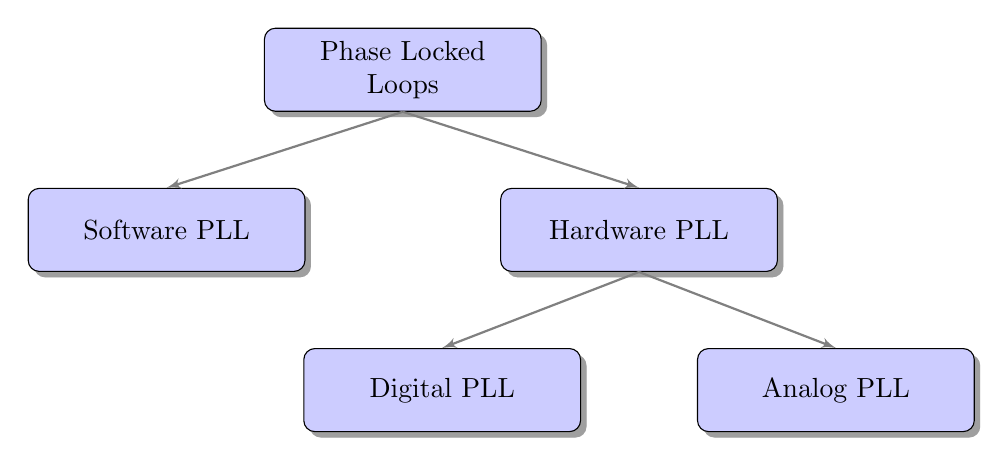
\begin{tikzpicture}[transform shape]
 
 % Draw diagram elements
  \path \myBlock {1}{Phase Locked Loops};
  \path (p1.south)+(-3,-1.5) \myBlock{2}{Software PLL};
  \path (p1.south)+(3,-1.5) \myBlock{3}{Hardware PLL};
  \path (p3.south)+(2.5,-1.5) \myBlock{4}{Analog PLL};
  \path (p3.south)+(-2.5,-1.5) \myBlock{5}{Digital PLL};
     
  % Draw arrows between elements
  \path [line] (p1.south) -- node  {} (p2.north);
  \path [line] (p1.south) -- node  {} (p3.north);
  \path [line] (p3.south) -- node  {} (p4.north);
  \path [line] (p3.south) -- node  {} (p5.north);

\end{tikzpicture}
\caption{A taxonomy of PLLs \cite{Best}}
\label{fig:Taxonomy}
\end{figure}

At this stage, it is important to elaborate on the taxonomy of PLLs, which can be visualised in figure \ref{fig:Taxonomy} and table \ref{tab:PLLTaxonomy}. The \ac{NAMURU} utilises a Software PLL, which is implemented in the C programing language on one of processor cores. However, in order to understand the operation and performance of the PLL, we analyse it as an Analog PLL. While every PLL is inherently non-linear, Gardner states that "Tools for analysis of nonlinear systems are exceedingly cumbersome and provide merger benefits compared to the powerful analytical tools available for linear systems". Gardner consistently states that linear methods are sufficient for the bulk of analysis and design of most PLLs, and therefore linear approximations should be employed wherever feasible\cite{Gardner}. 

\begin{table}[!htb]
\centering
\begin{tabular}{|l|l|l|l|}
\hline
\rowcolor[HTML]{C0C0C0} 
\begin{tabular}[c]{@{}l@{}}PLL Category\end{tabular}            & Phase Detector & Phase Error Signal & Loop Filter \\ \hline
\begin{tabular}[c]{@{}l@{}}LPLL (Linear PLL)\end{tabular}       & Analog         & Analog             & Analog      \\ \hline
\rowcolor[HTML]{EFEFEF} 
\begin{tabular}[c]{@{}l@{}}DPLL (Digital PLL)\end{tabular}      & Digital        & Analog             & Analog      \\ \hline
\begin{tabular}[c]{@{}l@{}}ADPLL (All Digital PLL)\end{tabular} & Digital        & Digital            & Digital     \\ \hline
\rowcolor[HTML]{EFEFEF} 
\begin{tabular}[c]{@{}l@{}}SPLL (Software PLL)\end{tabular}     & Software       & Software           & Software    \\ \hline
\end{tabular}
\label{tab:PLLTaxonomy}
\caption{A taxonomy of PLLs\cite{ADPLL,Best}.}
\end{table}

\clearpage

\section{Analog PLLs}
Analog PLLs provide a useful abstraction for the development and analysis of Digital PLLs. A common method of developing PLLs for \ac{GPS} receivers is to design the control loop in the Laplace (analog) domain, and convert it to the Z (digital) domain. 

\begin{figure}[!htb] 
    \centering
    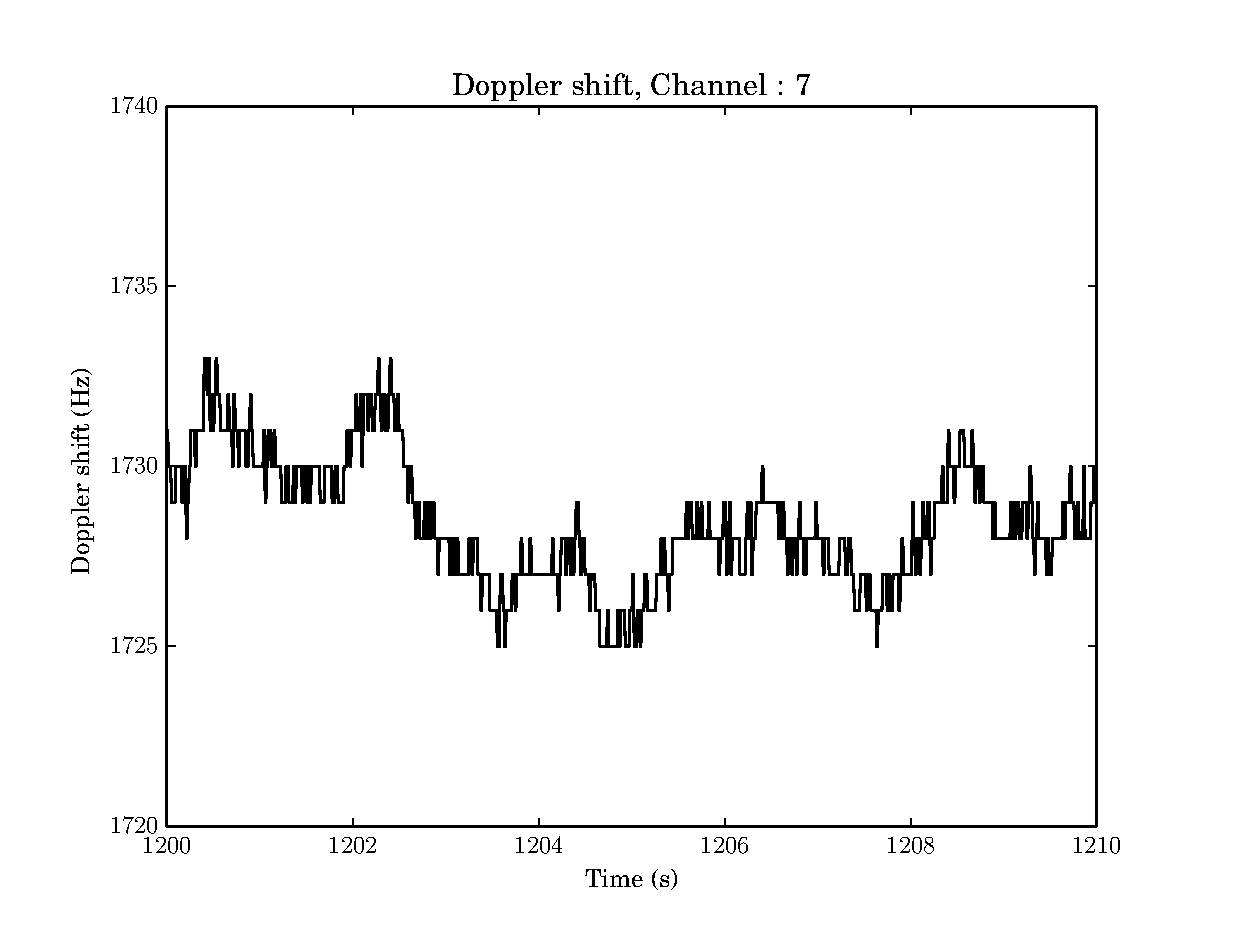
\includegraphics[width=1\textwidth]{LitReview/DopplerShift7.eps} 
    \caption{The raw output from the receiver while it is operating over a 10 second period. 
    The receiver is stationary, and tracking a live satellite.}
    \label{fig:DopplerShiftStationary}
\end{figure}

\begin{figure}[!htb] 
    \centering
    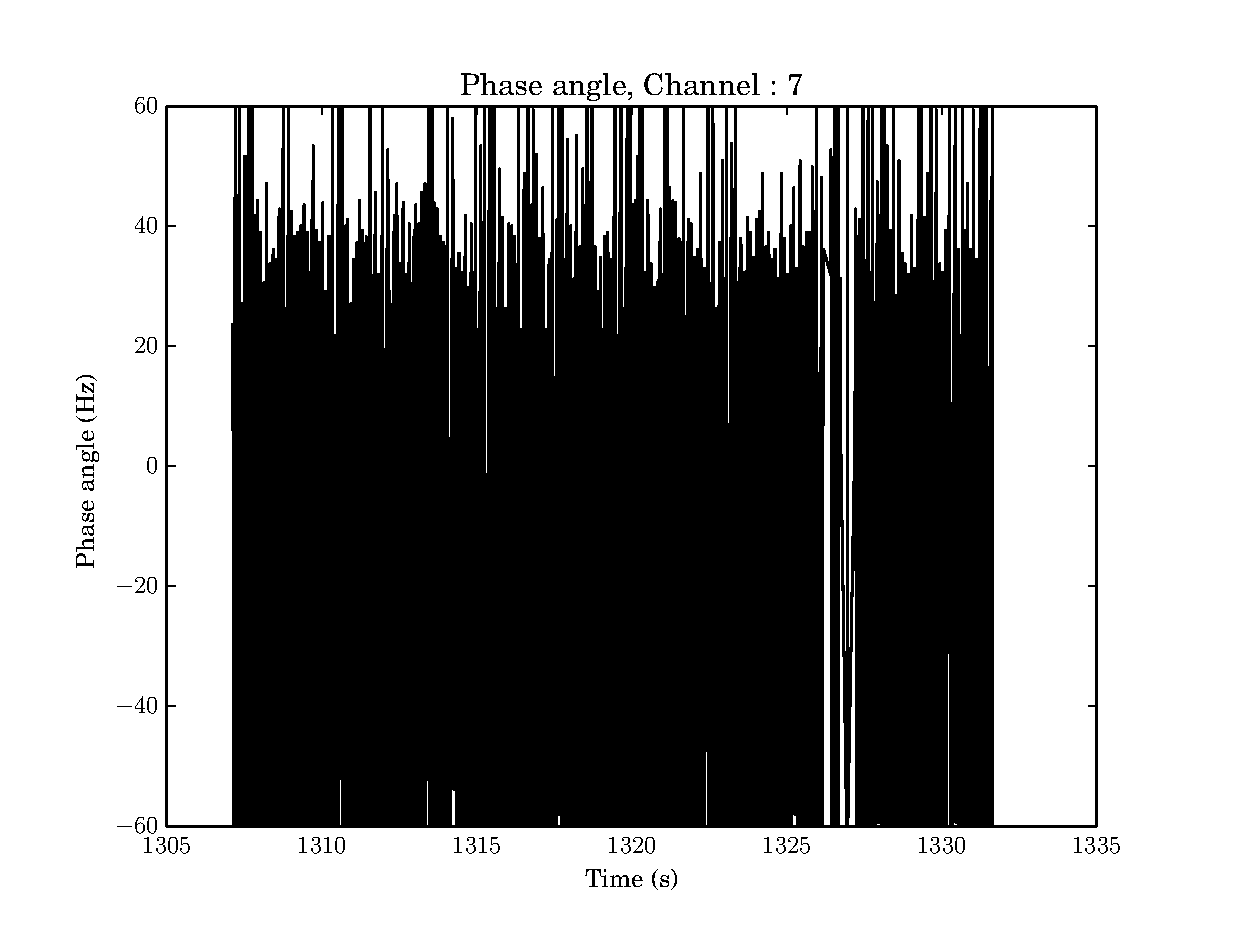
\includegraphics[width=1\textwidth]{LitReview/PhaseAngle7.eps} 
    \caption{The phase angle at the output from the phase detector while tracking the signal in figure \ref{fig:DopplerShiftStationary}. Note that the signal is zero mean.}
    \label{fig:PhaseAngleStationary}
\end{figure}

\begin{figure}[!htb] 
    \centering
    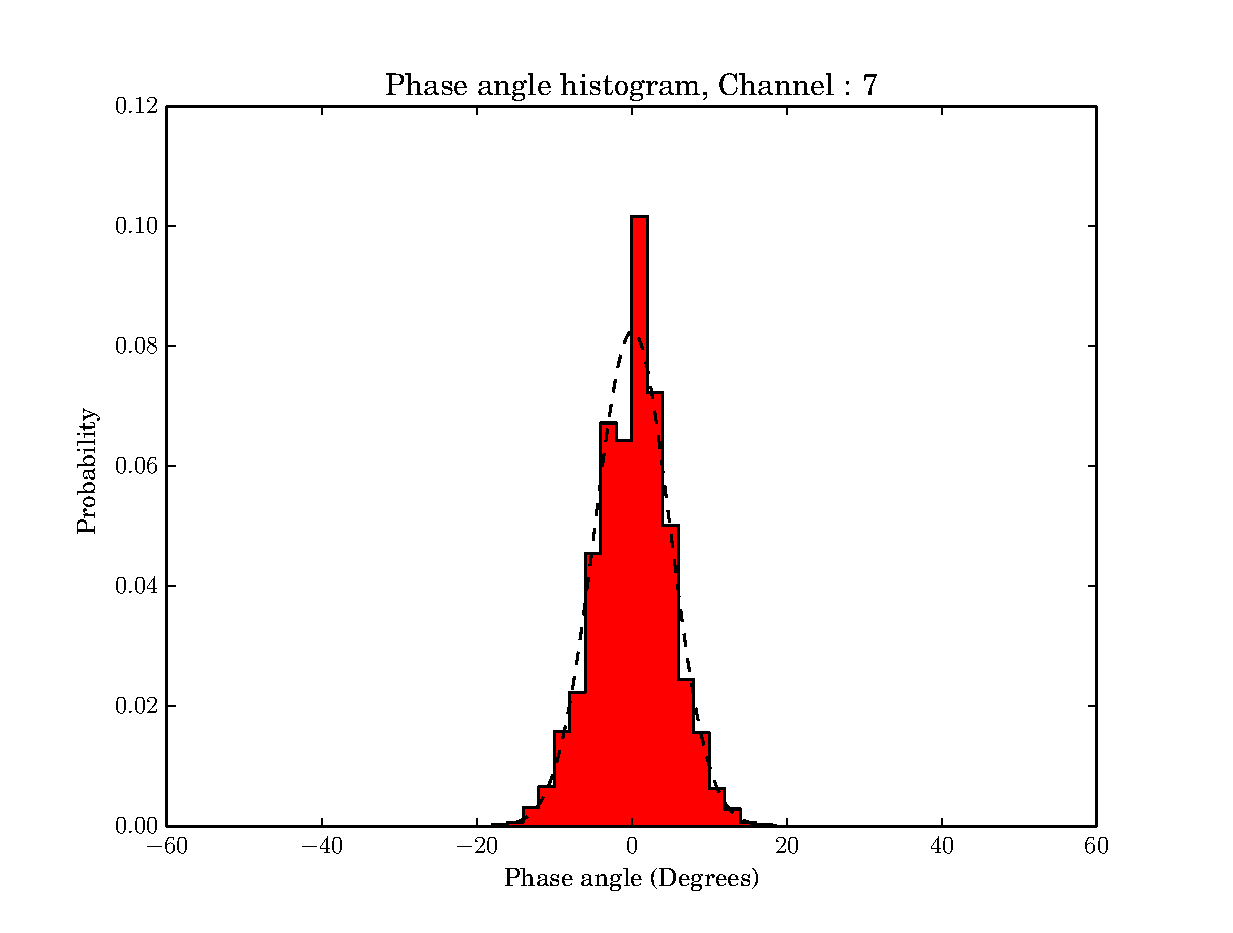
\includegraphics[width=1\textwidth]{LitReview/PhaseAngleHistogram7.eps} 
    \caption{A histogram of the phase angle from plot \ref{fig:PhaseAngleStationary}. A normal distribution with the 
    same mean (0) and standard deviation ($4.83\degree$) as the phase angle signal is overlaid. As will be discussed later, the standard deviation, $\sigma$ of the phase error is a crucial statistic in understanding the performance of a PLL tracking loop.}
    \label{fig:PhaseAngleHistogramStationary}
\end{figure}

	\subsection{Loop type}
    The choice of loop type is arguably the single most important choice that must be made
    during the design the tracking loops. The nomenclature of the term "loop type" is borrowed from control theory, 
    and refers to the number of integrators in the loop\cite{Gardner}. Because the \ac{VCO} is in effect an integrator,
    the order of a PLL is always at least 1. 
    
    From table \ref{tab:DopplerDynamics} we can see that the order of the dynamics the receiver
    experiences has and impact on the order of the Doppler shifts that will be seen by the receiver. Appendix \ref{ch:FlightDynamics}
    and \ref{ch:Falcon9} exhaustively analyse the dynamics that the \ac{LV} will experience, however in summary, the receiver will experience:
    
    \begin{enumerate}
    \item{Extreme velocities}
    \item{Persistent, significant acceleration}
    \item{Significant jerk}
    \end{enumerate}
    
    From table \ref{tab:LoopOrders} we can observe what order of dynamics different loop types are sensitive to. Ultimately, a trade-off exists between filter order and stability. Type 1 \& 2 filters are unconditionally stable in the Laplace domain, however they are not as effective as type 3 loops at coping with dynamics. For example, the residual error of a type 2 loop is acceleration. This makes it unsuitable for any application where sustained acceleration is likely to be encountered, as the error will increase over time, until phase lock is lost. However, type 2 are effectively insensitive to velocity, this is because the integrator in the loop filter contains and estimate of the Doppler shift due the current velocity. In most real world scenarios, sustained acceleration is limited, due to limits on maximum achievable velocities. For space based applications however, velocities of thousands of meters per second are routinely achieved. Hence while a type 2 loop may be suitable for terrestrial applications, a type 3 loop is typically required for spaced based applications. A type 3 loop is insensitive to acceleration and velocity, because the loop filter contains a pair of integrators. One of the integrators contains an estimate of the current velocity, the other of the current acceleration\cite{Kaplan}. 
    
    \begin{table}[!htb]
\centering
\begin{tabular}{|l|l|l|l|}
\hline
\rowcolor[HTML]{C0C0C0} 
Loop order & Filter order & Characteristics & Stability                               \\ \hline
1          & 0            & Sensitive to velocity stress       & Unconditionally stable                                  \\ \hline
\rowcolor[HTML]{EFEFEF} 
2          & 1            & Sensitive to acceleration stress   & Unconditionally stable                                   \\ \hline
3          & 2            & Sensitive to jerk stress          & Stable for $B_n$ \textless 18 Hz \\ \hline
\end{tabular}
\caption{Loop order behaviour. Note that the stability of the type 3 loop is predicated on a 20ms coherent integration time/update rate. The \ac{NAMURU} receiver uses an 8ms update rate, so the relevant loop bandwidth is 45Hz. Table from Kaplan\cite{Kaplan}.}
\label{tab:LoopOrders}
\end{table}

    
	\subsection{Stresses}
		\subsubsection{Thermal}
		\subsubsection{Dynamics}
		\ref{ch:FlightDynamics}
		\ref{ch:Falcon9}
		\subsubsection{Vibration}
		\ref{ch:Falcon9}
    \subsection{Noise bandwidth}
    
    
	\subsection{Loop coefficients}
	The determination of loop coefficients has been the subject of significant effort in the literature.  While the choice of loop type is relatively straightforward, and dictated by the application, the selection of appropriate coefficients for the loop filter is somewhat more nuanced. Hence, a focus of this thesis has been on critically analysing the loop coefficients used in the current \ac{NAMURU} receiver. 
	
	Kaplan describes the loop filter's objective as reducing noise, in order to produce an accurate estimate of the original signal\cite{Kaplan}. Gardner on the other hand takes a subtly different view, choosing to focus more on the loop filter's ability to regulate the output signal dynamics\cite{Gardner}. Again, it is important to recall at this point that the terms loop filter and loop controller are synonymous. 
	
	
	The \ac{NAMURU} receiver uses a number of different PLL's while in different operational states. The relationship between the different types of PLL's used as further analysis is carried out in appendix \ref{ch:StateTransitions} and \ref{ch:LaplaceAnalysis}. The state that will receive the most thorough analysis in this thesis is the type 3 PLL. 
	
	
	From Gardner, we find that we can require 3 independent parameters in order to characterise the PLL\cite{Gardner}. In equation \ref{eq:3rdOrderLoop}, we can observe the presence of $s^3$ in the denominator, confirming that this is a type 3 loop. The factor of $\frac{1}{s}$ is the integrator inside the \ac{VCO}.
	
	
	\begin{equation}
	G(s) = \frac{1}{s}(1 + \frac{K_2}{K_1s} + \frac{K_3}{K1s^2})
	\label{eq:3rdOrderLoop}
	\end{equation}
	
	
	The design method which was used to originally design \ac{NAMURU} is described by Ward and Kaplan, \cite{Ward,Kaplan}, and relies on designing the PLL in the Laplace (analog) domain, and then transforming into the digital domain for implementation. The method developed by Ward enjoys significant popularity, in part because it develops relatively robust designs, based on proven rules of thumb. The design process used will be described in more comprehensive detail in chapter \ref{ch:MyWork}, however it is important to recognise other design methods that exist. 
	\subsection{Stability}

\clearpage

\section{Digital PLL's}
	\subsection{Integrators}
	One of the most important aspects of the digital design is the method used to transform integrators the the Laplace domain to the Z domain. The Aquarius firmware\cite{FirmwareCode} written by Glennnon extensively uses the boxcar transform. The boxcar integrator is also used by Van Dierendonck  \cite{Spilker} in his GPS architecture. Conversely, Kaplan \cite{Kaplan} demonstrates an implementation of a tracking loop using Ward's parameters using bilinear integrators. The important and effect of using different integrators will be discussed more thoroughly in \ref{ch:MyWork}.
	
	\subsection{Stability}
	    While analysis in the S domain is instructive, further analysis of stability in the Z domain is authoritative in the design process. Gardner 
	    
	    Kaplan's contribution to an understanding of stability is somewhat limited. While he provides a formulaic approach to designing tracking loops, the reader is warned that the loop noise bandwidth of a type 3 PLL must not exceed 18Hz\cite{Kaplan}. The reasoning behind this statement is explored in more detail by Kazemi, who spends significant effort analysing the effect of sampling time on the stability of the PLL. In summary, with a sufficiently high loop bandwidth time product, the closed poles of the transfer function will migrate outside the unit circle. As discussed at length in Gardner \cite{Gardner}, this leads to instability. 
	    